\documentclass[12pt, a4paper]{article}

\usepackage{xeCJK}
\usepackage{fontspec}
\usepackage{indentfirst}
\usepackage{booktabs}
\usepackage{fancyhdr}
\usepackage{graphicx}
\usepackage{listings}
\usepackage{xcolor}
\usepackage{amsmath}
\usepackage{amsfonts}
\usepackage{amssymb}
\usepackage{amsthm}
\usepackage{multirow}
\usepackage[margin=1.25in]{geometry}

\pagestyle{fancy}
\setmainfont{思源宋体 CN}
\setmonofont{Inziu Iosevka SC}
\setCJKmainfont{思源宋体 CN}
\setCJKmonofont{Inziu Iosevka SC}
\linespread{1.5}

\lstset{
    basicstyle=\footnotesize\ttfamily,
    keywordstyle=\bfseries,
    numbers=left,
    frame=single,
    columns=fixed,
    showspaces=false,
    showstringspaces=false,
    language=java,
    breaklines=true
}

\renewcommand\contentsname{目录}

\begin{document}

\begin{titlepage}
\begin{center}

% Upper part of the page

\includegraphics[width=0.15\textwidth]{../assets/logo.jpg}\\[1cm]

\textsc{\LARGE 东南大学} \\[1.5cm]
\textsc{\Large 计算机科学与工程学院} \\[0.5cm]

% Title
{\rule{\linewidth}{1mm}}\\[0.4cm]
{\huge \bfseries 语法分析实验报告} \\[0.4cm]
{\rule{\linewidth}{0.5mm}}\\[1.5cm]

% Author and supervisor
\begin{minipage}{0.4\textwidth}
\begin{flushleft}
\large
作者:\\
学号:
\end{flushleft}
\end{minipage}
\begin{minipage}{0.4\textwidth}
\end{minipage}
\begin{minipage}{0.4\textwidth}
\begin{flushright}
\large
课程:编译原理
\end{flushright}
\end{minipage}

\vfill

% Bottom of the page
{\large 2018.1}

\end{center}
\end{titlepage}
 % 标题页

\tableofcontents
\newpage

\section{介绍}
本次实验选择C的子集Mini-C构造一个语法分析器

\section{词法语法描述}
\subsection{C11规范}
C11规范来自于cppreference\footnote{http://en.cppreference.com} 中所列举的C语言结构描述。Mini-C从中选取了常用的关键字来构成 C 语言的子集,包括数字、常用的数据类型、条件控制语句、\verb|For|循环、和常见的运算操作符与函数调用。为了表示的简洁性,本次实验只保留条件控制语句。本次报告的示例程序如下所示。
{\linespread{1}
\begin{lstlisting}[caption=本次实验的实验用例]
if (i)
    if (j)
        a;
    else
        b;
else
    if (k)
        d;
\end{lstlisting}}
\subsection{Mini-C正规式描述}
参照C11规范,我们得到Mini-C的词法正规式。
{\linespread{1}
\begin{lstlisting}[caption=Mini-C的词法正规式]
delim       [ \t\n]
ws          {delim}+
digit       [0-9]
digits      {digit}+
number      {digits}(\.{digits})?([Ee][+-]?{digits})?
symbol      "("|")"|"{"|"}"|";"|"["|"]"|","
letter_     [A-Za-z\_]
id          {letter_}({letter_}|{digit})*
str         \"[^\"]*\"
comparison  "<"|">"|"<="|">="|"=="|"!="
operator    "+"|"-"|"*"|"/"|"="|"++"|"--"|"<<"|">>"|"||"|"&&"
\end{lstlisting}}
有一些简单的正则表达式模式,比如~\verb|if|。如果我们在输入中看到两个字母~\verb|if|,并且~\verb|if|之后没有跟随其他字母和数字,就会返回词法单元~\verb|IF|。这样的保留字我们用一个保留字表来维持,在获得词素之后参照保留字来判断词法单元是什么。其他关键字处理方式与之类似。
{\linespread{1}
\begin{lstlisting}[caption=Mini-C的关键字]
if else for void char int return
\end{lstlisting}}
\subsection{BNF范式}
下面给出Mini-C的BNF范式
\begin{align*}
    \text{S } & \rightarrow \text{ if B S}\\
    \text{S } & \rightarrow \text{ if B S else S}\\
    \text{S } & \rightarrow \text{ id ;}\\
    \text{B } & \rightarrow \text{ ( id )}
\end{align*}
\subsection{LR(1)项集}
详见第\pageref{fig:LR1}~页附录\ref{sec:LR1}~图\ref{fig:LR1}。
\subsection{LR(1)分析表}
详见第\pageref{fig:LR1table}~页附录\ref{sec:LR1table}~表\ref{fig:LR1table}。

\section{语法分析程序}
项目复用了前一次语法分析实验的内容,在LexicalAnalysis\footnote{https://github.com/shellqiqi/LexicalAnalysis} 中描述了词法分析的细节,本节不介绍相关的代码细节。
\subsection{程序结构}
本程序分两个包,\verb|lexer|包包含词法分析类,\verb|parser|包包含语法分析类,\verb|App|作为入口类。\verb|lexer|中有三个类,\verb|DFA|类从~\verb|resource|中读取一个状态转化表,\verb|Lexer|类做词法分析,\verb|Token|是一个词素。\verb|parser|中有四个类,\verb|Parser|类做语法分析并给出语法分析树,\verb|SyntaxTree|类由~\verb|SyntaxTreeNode|类与~\verb|TokenNode|类组合而来,表示一个语法分析树。资源文件包括一个由Mini-C编写的程序以及识别语言的状态转化表。
\subsection{语法分析树数据结构}
\begin{figure}[htbp]
    \centering
    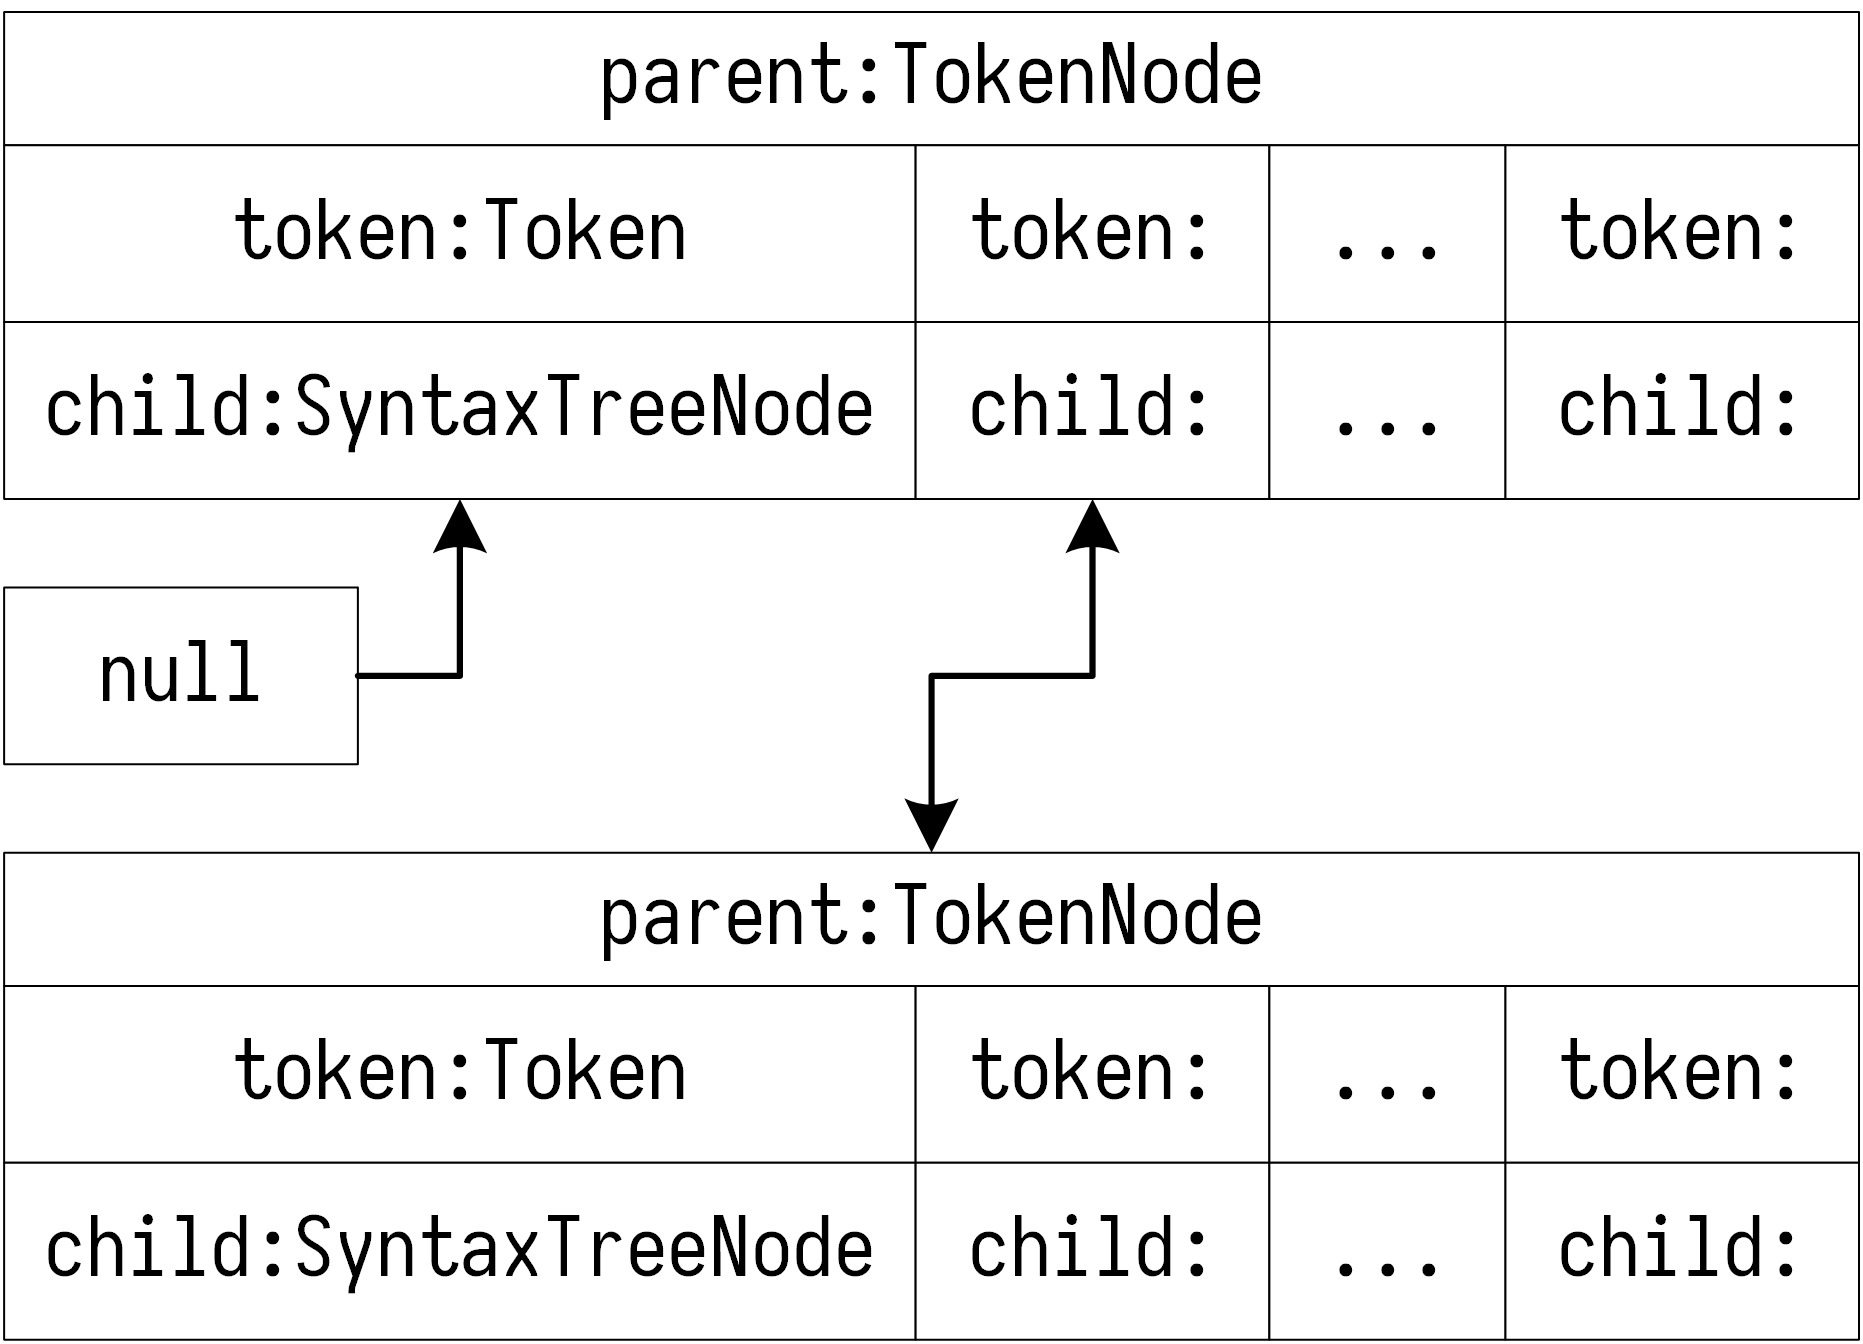
\includegraphics{../assets/SyntaxTree.png}
    \caption{语法分析树数据结构}
\end{figure}
\subsection{程序源码}
\subsubsection{\texttt{Parser}类程序清单}
{\linespread{1}
\lstinputlisting[caption=Parser.java]{../src/main/java/shell7/parser/Parser.java}}
\subsubsection{\texttt{SyntaxTree}类程序清单}
语法分析树类保存了树的根节点和根上~\verb|Token|列表的栈操作。
{\linespread{1}
\lstinputlisting[caption=SyntaxTree.java]{../src/main/java/shell7/parser/SyntaxTree.java}}
\subsubsection{\texttt{SyntaxTreeNode}类程序清单}
语法分析树结点保持了该结点的亲属和一个~\verb|Token|列表。
{\linespread{1}
\lstinputlisting[caption=SyntaxTreeNode.java]{../src/main/java/shell7/parser/SyntaxTreeNode.java}}
\subsubsection{\texttt{TokenNode}类程序清单}
\verb|Token|结点保持了一个终结符或一个非终结符的一个展开。
{\linespread{1}
\lstinputlisting[caption=TokenNode.java]{../src/main/java/shell7/parser/TokenNode.java}}
\subsection{测试结果}
{\linespread{1}
\begin{lstlisting}[caption=本次实验的实验用例]
S
S -> IF B S ELSE S
    B -> ( ID )
    S -> IF B S ELSE S
        B -> ( ID )
        S -> ID ;
        S -> ID ;
    S -> IF B S
        B -> ( ID )
        S -> ID ;
\end{lstlisting}}
% \include{section/section4}

\appendix
\section{LR(1)项集}\label{sec:LR1}
\begin{figure}[htbp]
    \centering
    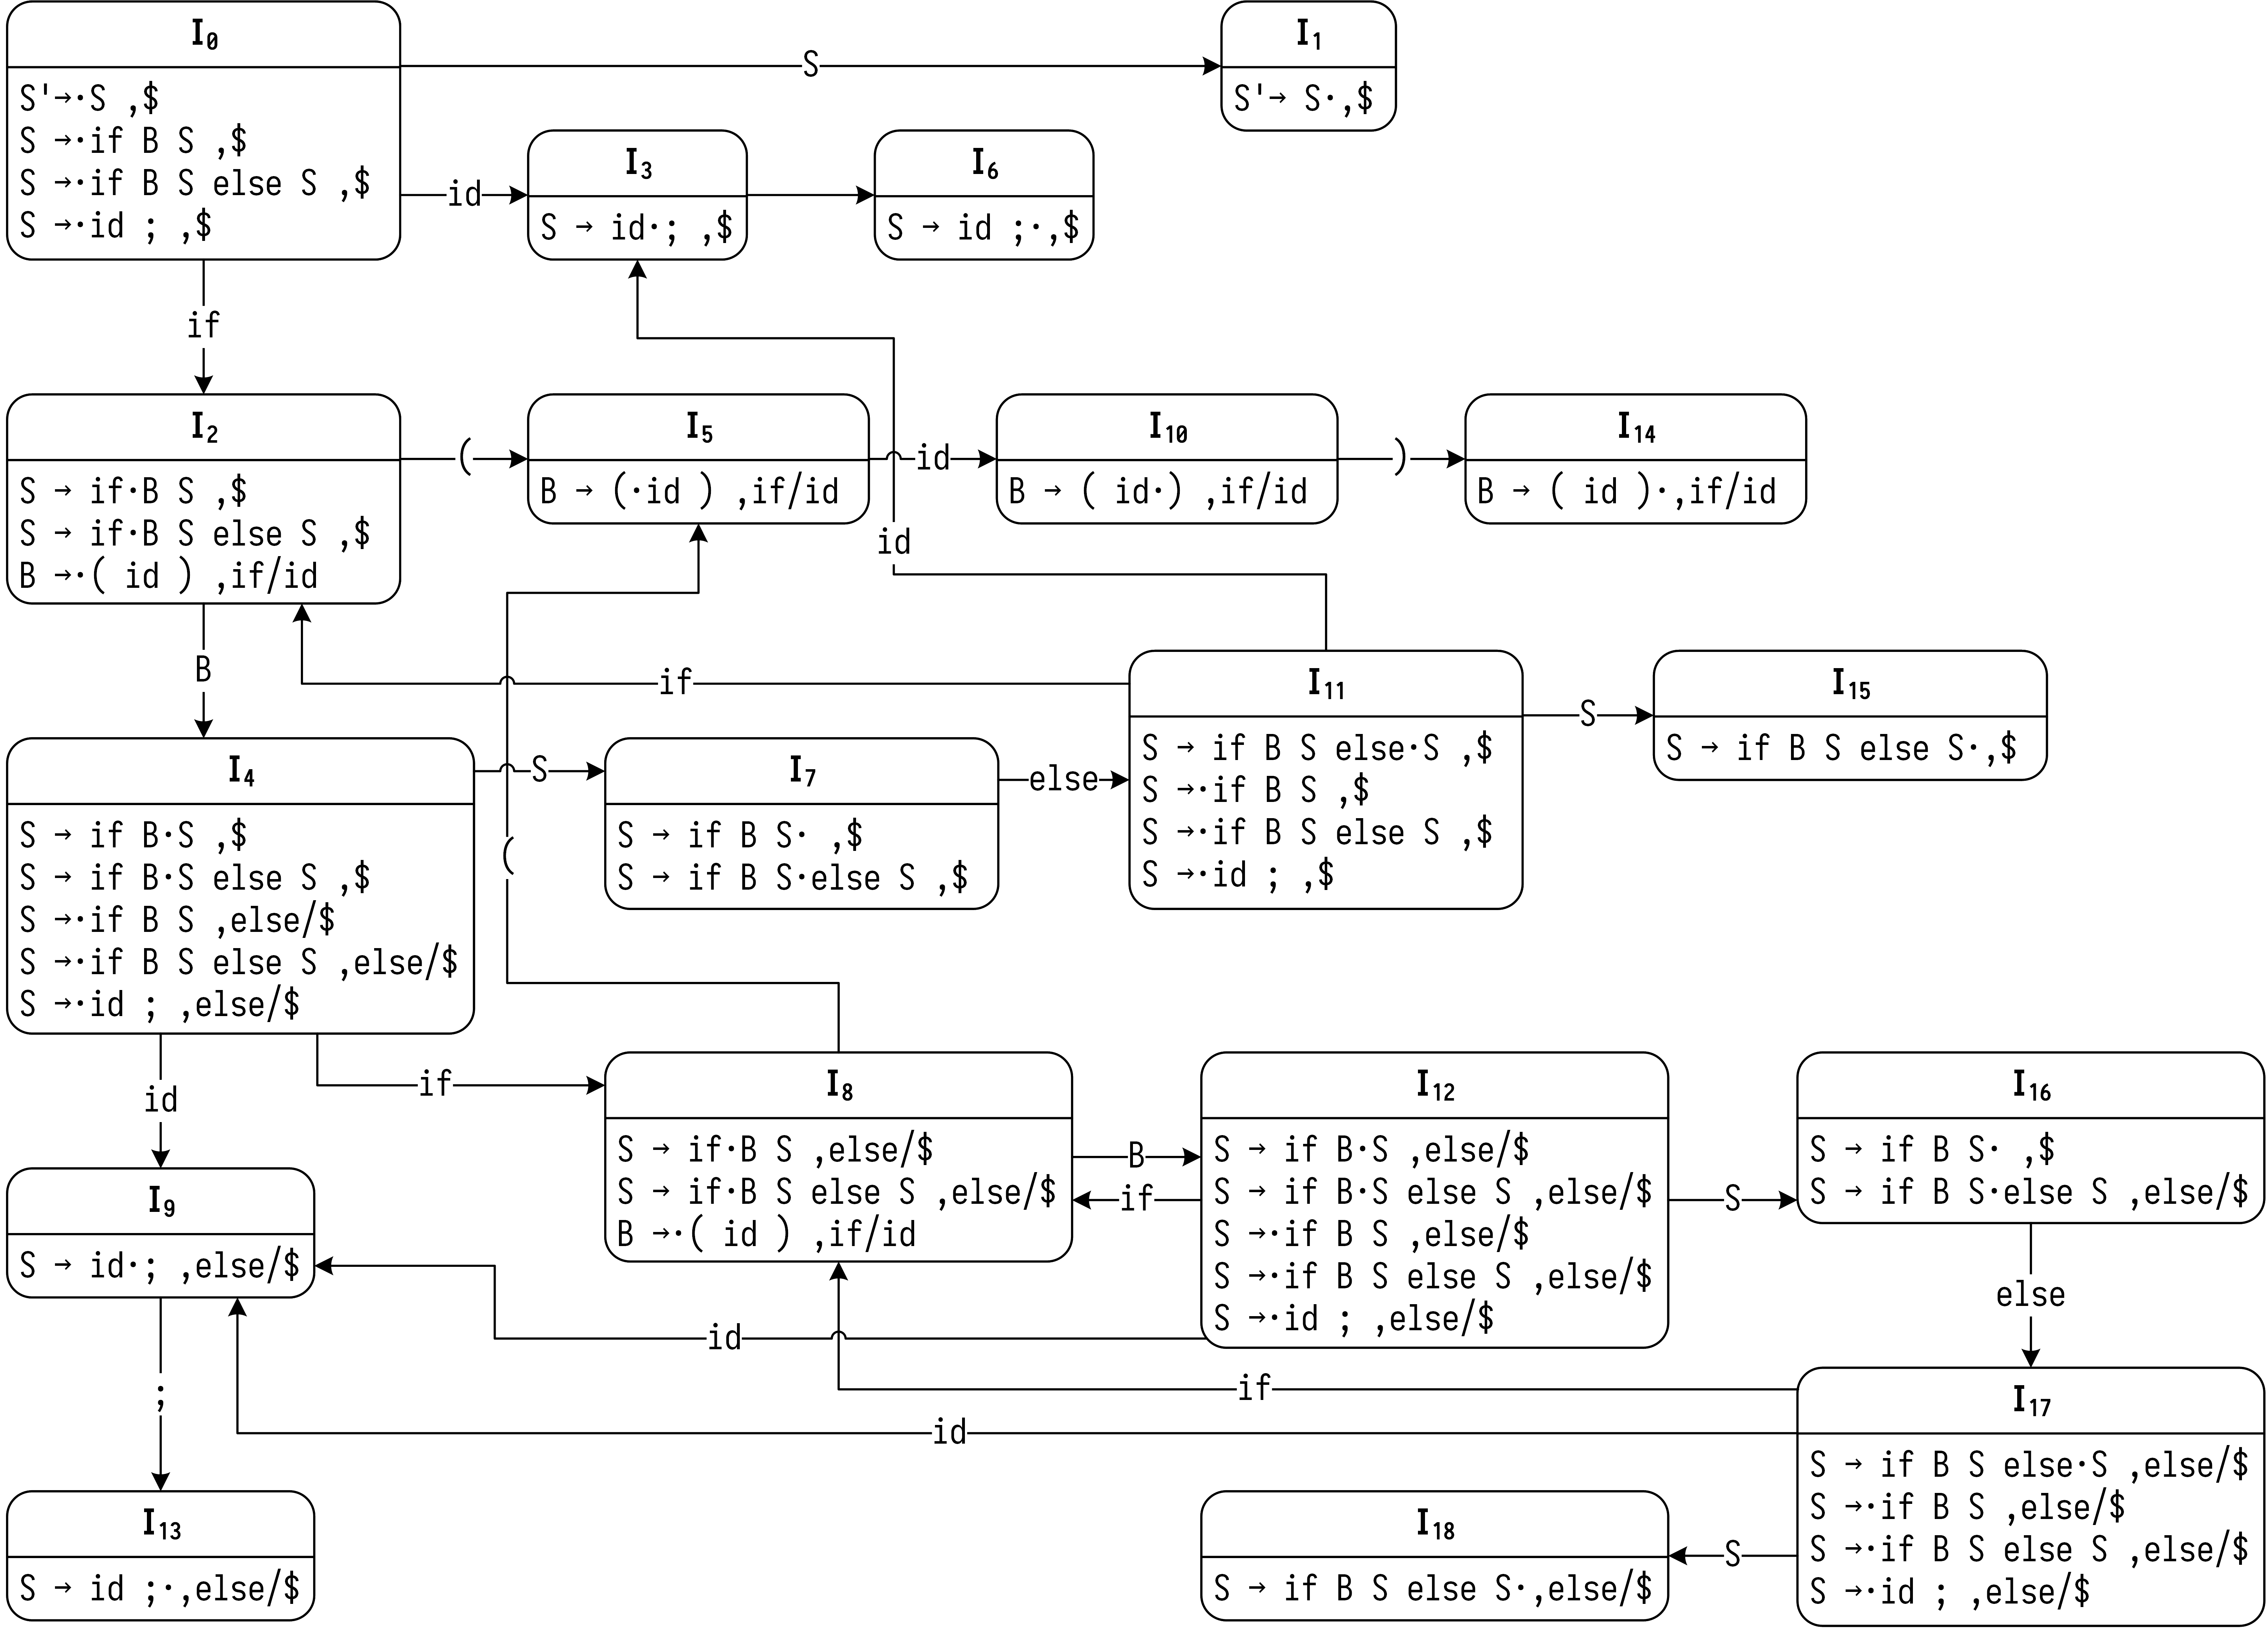
\includegraphics[scale=0.6,angle=90]{../assets/LR1.png}
    \caption{LR(1)项集}\label{fig:LR1}
\end{figure}

\section{LR(1)分析表}\label{sec:LR1table}
\begin{table}[!h]
    \centering
    \begin{tabular}{c | c c c c c c c | c c}
        \toprule
        \multirow{2}{*}{status} & \multicolumn{7}{| c |}{ACTION} & \multicolumn{2}{c}{GOTO}\\
        \cline{2-10}
        & if & id & ( & ) & ; & \$ & else & S & B\\
        \hline
        0  & s2 & s3  &    &     &     &     &     & 1  &   \\
        1  &    &     &    &     &     & acc &     &    &   \\
        2  &    &     & s5 &     &     &     &     &    & 4 \\
        3  &    &     &    &     & s6  &     &     &    &   \\
        4  & s8 & s9  &    &     &     &     &     & 7  &   \\
        5  &    & s10 &    &     &     &     &     &    &   \\
        6  &    &     &    &     &     & r4  &     &    &   \\
        7  &    &     &    &     &     & r1  & s11 &    &   \\
        8  &    &     & s5 &     &     &     &     &    & 12\\
        9  &    &     &    &     & s13 &     &     &    &   \\
        10 &    &     &    & s14 &     &     &     &    &   \\
        11 & s2 & s3  &    &     &     &     &     & 15 &   \\
        12 & s8 & s9  &    &     &     &     &     & 16 &   \\
        13 &    &     &    &     &     & r4  & r4  &    &   \\
        14 & r3 & r3  &    &     &     &     &     &    &   \\
        15 &    &     &    &     &     & r2  &     &    &   \\
        16 &    &     &    &     &     & r1  & s17 &    &   \\
        17 & s8 & s9  &    &     &     &     &     & 18 &   \\
        18 &    &     &    &     &     & r2  & r2  &    &   \\
        \bottomrule
    \end{tabular}
    \caption{LR(1)分析表}\label{fig:LR1table}
\end{table}


\end{document}